The interstellar medium (ISM) is the material within a galaxy between the stars \citep{mckee_dynamical_1999}. The cold, dense regions of the ISM, mostly composed of molecular hydrogen, are known as molecular clouds. Figure \ref{fig: molecular_cloud} shows the structure of a molecular cloud, which have sub-regions of higher densities.  Within clumps and filaments of material are dense cores (brown ovals in Figure \ref{fig: molecular_cloud}), which are typically < 0.1 pc in size.  When these cores become gravitationally unstable, they collapse under their own gravity, marking the beginning of the star formation process \citep{Kuruwita}. 



% ------------------------------------------------
\begin{figure}[htbp]
  \centering
  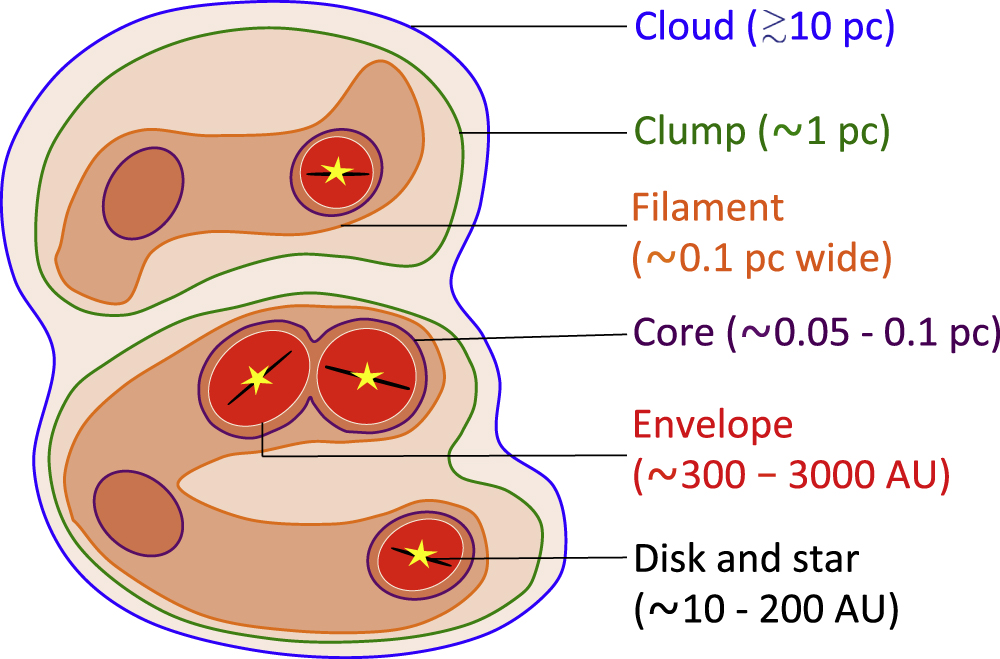
\includegraphics[width=0.5\textwidth]{WRITEUP_AND_IMAGES/IMAGES/WRITEUP/NOTMINE/apjaaa240f1_hr.jpg}
  \caption[Cartoon schematic of the structure inside a molecular cloud.]{Cartoon schematic of the structure inside a molecular cloud.  The image is from \cite{Pokhrel}. \permission{Ask for permission}}
  \label{fig: molecular_cloud}
\end{figure}
% ------------------------------------------------
As a core collapses and forms a protostar at its center, a circumstellar disk can form around the young star as a result of conservation of angular momentum \citep{Williams}. Figure \ref{fig: YSO} gives a broad overview of young stellar object (YSO) evolution. During the Class 0 stage, the young protostar and disk are deeply embedded within a surrounding envelope of gas and dust, which contains most of the system's mass \citep{Williams, Kuruwita}. As material from the envelope is accreted onto the disk and protostar, the envelope begins to dissipate and the system evolves into the Class I stage \citep{Williams}. During this stage, the disk is still embedded in the envelope, but the envelope's mass is comparable to, or lower than, the disk mass \citep{Kuruwita}. By the Class II stage, most of the system's mass is in the central star and the envelope is mostly dispersed. A gaseous disk remains, but its mass is much lower compared to the mass of the central star. In the Class III stage, the envelope has dispersed, the disk has negligible mass, and the central star is a pre-main
sequence object \citep{Kuruwita}. 



% ------------------------------------------------
\begin{figure}[htbp]
  \centering
  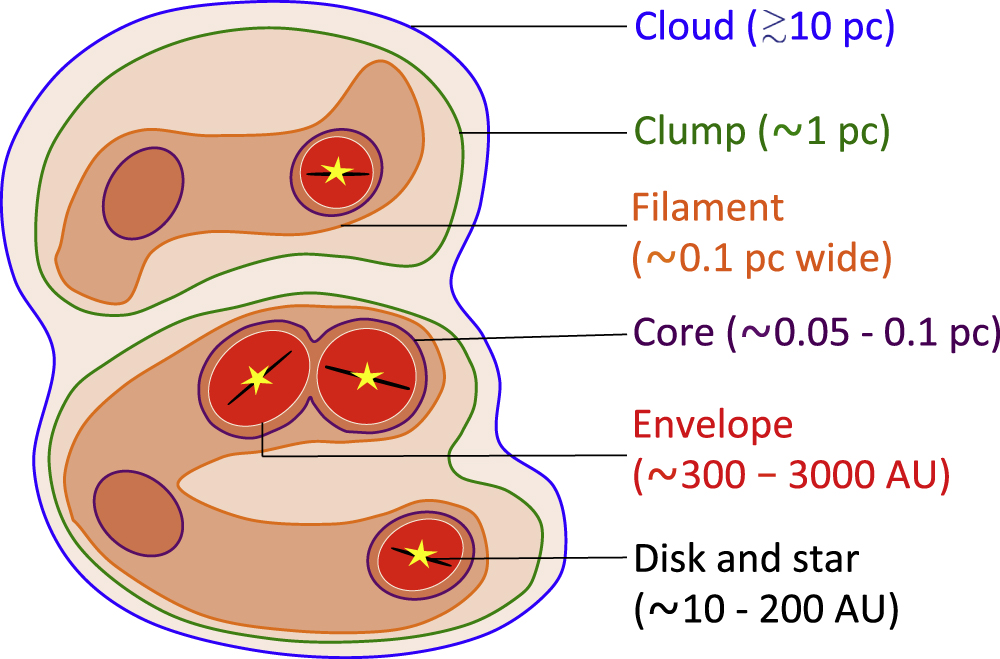
\includegraphics[width=0.5\textwidth]{WRITEUP_AND_IMAGES/IMAGES/WRITEUP/NOTMINE/apjaaa240f1_hr.jpg}
  \caption[ADD]{\add{Caption} \coded{Added image} \permission{Ask for permission}}
  \label{fig: YSO}
\end{figure}
% ------------------------------------------------




%------------------------------------------------
\begin{figure}[htbp]
  \centering
  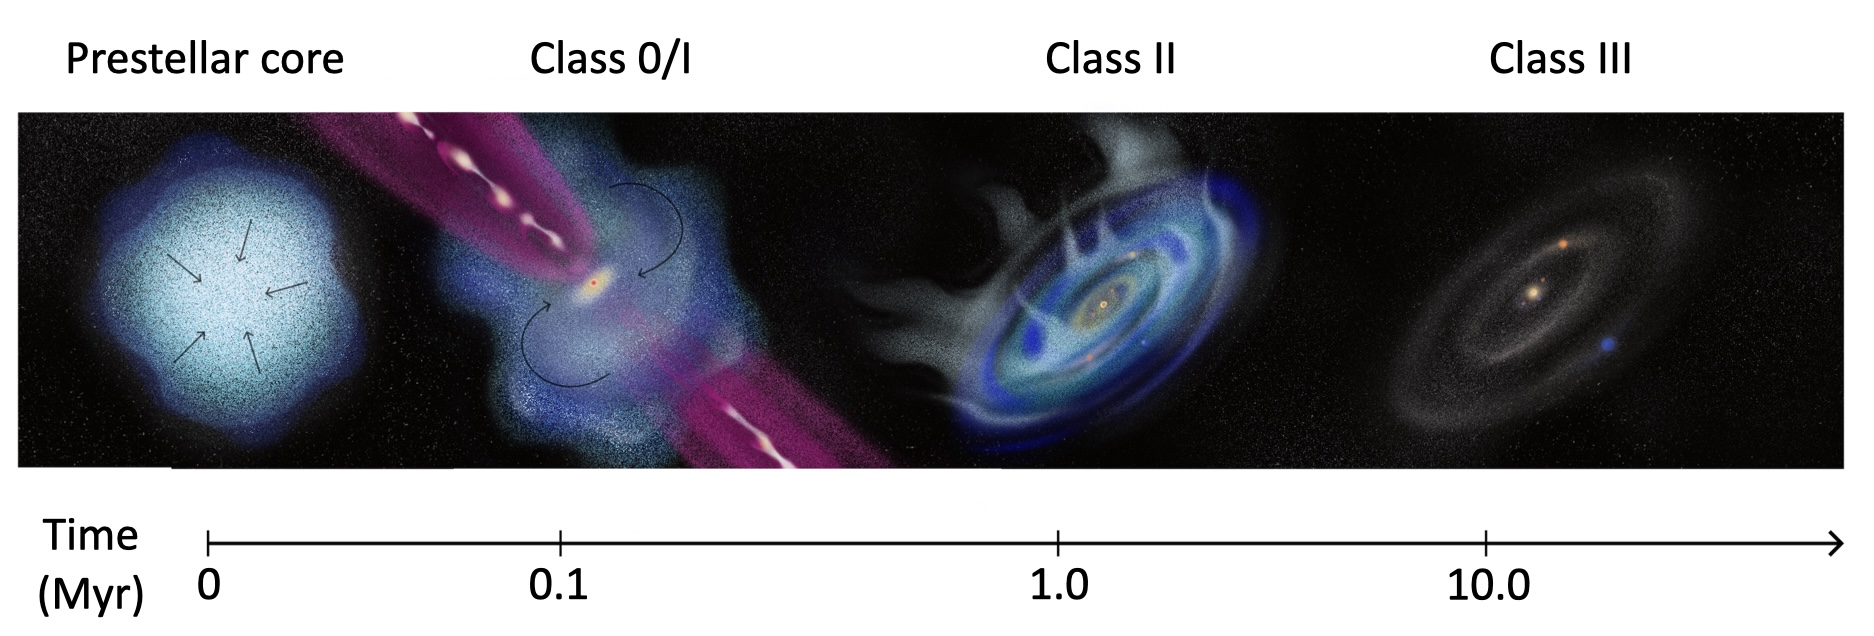
\includegraphics[width=0.99\textwidth]{WRITEUP_AND_IMAGES/IMAGES/WRITEUP/NOTMINE/classes_v2.jpeg}
  \caption[Overview of protostellar evolutionary phases.]{Overview of protostellar evolutionary phases. Image from \cite{Kuruwita}. \permission{Ask for permission} }
  \label{fig: star-formation-schematic}
\end{figure}
% ------------------------------------------------

Overall, the evolutionary Classes generally correspond to an evolutionary sequence where more evolved systems have less material in the surrounding envelope and disks. \ref{fig: star-formation-schematic} illustrates the various evolutionary stages from a prestellar core to a Class III disk. 







